\subsection{Chromatic Adaptation and Colour Constancy}

\textit{Shortly after the start of my PhD program I attended a symposium for PhD students in the field of lighting research (LumeNet). At this symposium Prof. Michael Pointer delivered a welcome talk, and one particular part of it stuck with me.}

\textit{He described how at the start of his PhD studies \citep{pointer_colour_1972}, he had made copies of every paper which had been written on his subject (Chromatic Adaptation) which were available from the library, and written to any authors whose work he had been unable to access, requesting copies. At the end of his first year he had a binder which contained, as far as he was aware, everything ever written on the subject. He finished his story rather abruptly, along the lines of ``since then, so many people have written on the subject that it would take much longer than you have within a PhD program to read it all. I don't know what you all will do''. Not an encouraging thought!}

\textit{With this in mind, I shall attempt only to cover the basics and a few select papers of particular relevance in the following section, and shall take this opportunity to note my debt to a number of comprehensive overview papers and book chapters on this subject: \citet{foster_color_2011,smithson_sensory_2005,hurlbert_computational_1998,brainard_color_2014,fairchild_color_2013}.}

\subsubsection{The problem}

At the start of this section I stated that ``Our perception of colour generally correlates with the way in which objects preferentially reflect some wavelengths over others''. It transpires that this ability is non-trivial, because our visual systems do not have access to the \glspl{SRF} of the objects which are seen, only the levels to which retinal cells are excited, which depends on the interaction of illuminant, surface and sensor. 

Figure \ref{fig:problem} demonstrates the problem, by reproducing Figure \ref{fig:1931} with a minor adjustment; where the previous figure had the chromaticities of the set of surfaces under only a single illuminant, a large number of illuminants are used here. It can be seen that it is not uncommon for one surface to have a chromaticity under one illuminant that another surface has under a different illuminant. Thus, the relationship between surface and chromaticity appears to break down.

\begin{figure}[htbp]
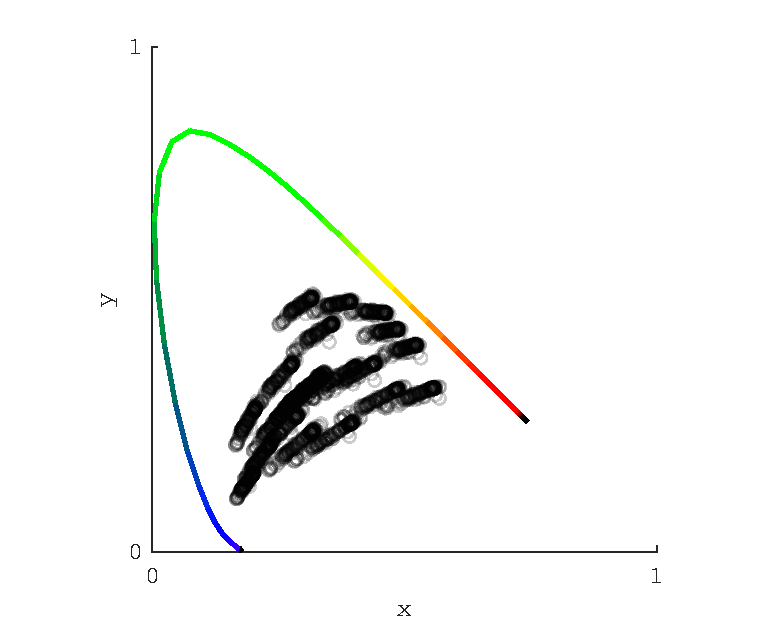
\includegraphics[max width=\textwidth]{figs/LitRev/ColorimetryDemo6.pdf}
\caption{A reproduction of Figure \ref{fig:1931}, but this time with the chromaticity co-ordinates for the 24 macbeth colour checker patches under a range of daylights, drawn from the Granada dataset \citep{hernandez-andres_color_2001} (further described in Section \ref{sec:coldata}).}
\label{fig:problem}
\end{figure}

In order to provide a representation of colour where the perceived colour remains constant across changes in illuminant (thus the term \emph{colour constancy}), the human visual system must find a way to solve this problem.

\subsubsection{Adaptation}

`Adaptation' is the general mechanism by which a finite range of sensitivity can be shifted in terms of absolute sensitivity bounds. The benefit of having an adaptive system, as opposed to a fixed system, is that the sensitivity of the system to small changes is maximised, whilst maintaining a broad overall sensitivity, at the expense of being able to sense over the entire range at a single time-point. 

\begin{figure}[htbp]
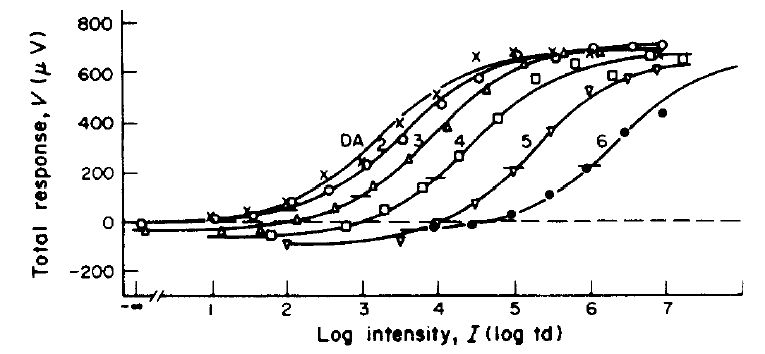
\includegraphics[max width=\textwidth]{figs/LitRev/Valeton.png}
\caption{Cone flash response at different levels of adaptation in macaques, reproduced from \citet{valeton_light_1983}. On the left `DA' stands for dark-adapted, with the rising numbers for the other lines relating to rising adapting levels.}
\label{fig:Valeton}
\end{figure}

In an environment such as the terrestrial environment, there is a great range in the level of illumination, but this range is rarely existent contiguously; levels of illumination tend to be similar across a scene, and only change rather slowly over time. The notable exception, and thus where we notice the expense of having an adaptive visual system, comes when we enter or exit an environment where illumination is almost entirely excluded, such as a dark cave or below-decks of a boat. 

Where the process of adaptation responds to overall illumination levels, it is referred to as light adaptation and dark adaptation. Where the process of adaptation responds to the wavelength composition of light reaching the eye it is referred to as chromatic adaptation.

In a natural environment, a change in the wavelength composition of radiation reaching the eye from a specific object might be caused by changing weather or time of day, or by the physical movement of the object from one space to another (where different lighting exists in the two different spaces). Figure \ref{fig:SPDnorm} shows a set of \glspl{SPD}, normalised by luminance, showing that the wavelength composition varies quite considerable, though in relatively systematic fashion.

\begin{figure}[htbp]
%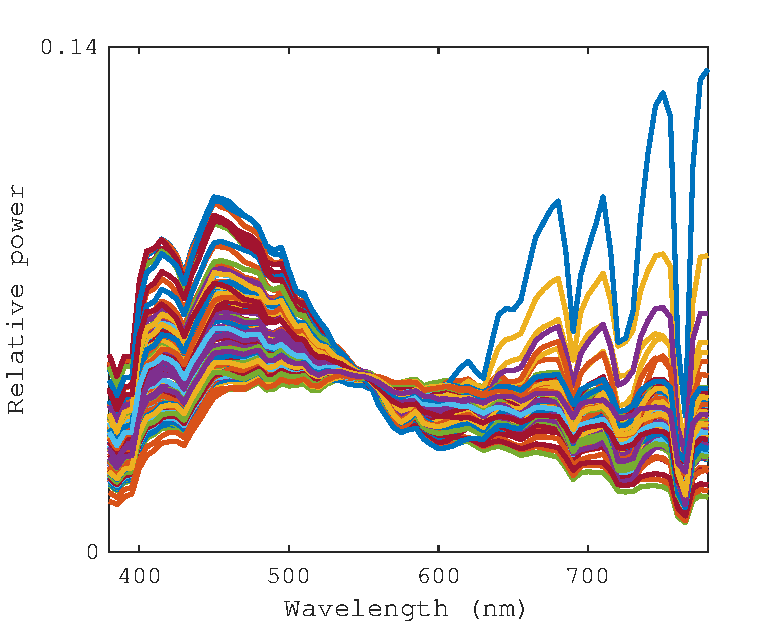
\includegraphics[max width=\textwidth]{figs/LitRev/ColorimetryDemo7.pdf}
\caption{The \glspl{SPD} of a subset of the daylight measurements of \citet{hernandez-andres_color_2001} (further described in Section \ref{sec:coldata}), normalised by luminance.}
\label{fig:SPDnorm}
\end{figure}

\subsubsection{Mechanistic vs. Inferential}

In the literature there seems to be a long-running grapple between colour constancy and chromatic adaptation, with blurred boundaries and mixed definitions occurring frequently. \citet{brill_chromatic_1986} drive a wedge between the two concepts, asserting that the two operate on different timescales and in different fashions. The most common uses of the terms now seem to be for chromatic adaptation to refer to low level adaptation, with \citet{brainard_color_2014} using the term `mechanistic' to refer to this type of transformation.

\begin{citequote}{brainard_color_2014}
Adaptation of this sort supports constancy to the extent that its overall effect is to stabilize the postreceptoral representation of the light reflected from objects across changes of illumination (as well as other contextual changes).
\end{citequote}

The term `colour constancy', by contrast, is used to refer to higher level inference-based processes, which occur at faster timescales than are possible by adaptation alone \citep{rinner_time_2000}.

\subsubsection{von Kries Adaptation}

The conceptually simplest model of chromatic adaptation, and the forefather of many other models, is that referred to as Von Kries adaptation.

Johannes von Kries was one of the first to deeply consider chromatic adaptation, and appears to have understood it as a problem of sensory adaptation. In his formative series of papers, available in translation \citep{von_kries_beitrag_1970}, he laid out how the study of chromatic adaptation could be divided into two broad and complementary aims. 

The first referred to the systematic representation of the transforms in sensation caused by specific adaptations, such that \textit{``for any light mixture stimulating the readapted part [of the retina], another light mixture is specified that stimulates the same sensation is a normally adapted part \dots The purpose of this study would be solved completely if a general rule could be obtained for the effects of all possible adaptions.''} The search for `corresponding colours' (pairs of colours which match under asymmetric adaptation states), and for suitable systems to predict the appearance of colours in all situations, fall within this category of exploration. Out of this aim grew the study of \glspl{CAT}, where the search for an algorithm which would mathematically predict the locations in colour space of corresponding colours has been the fundamental goal \citep{cie_cie_2004-1}.

von Kries suggested that the second categorical aim of chromatic adaptation research ought to be to discover `how the adaptation is produced by exposure to any particular color, continued over an extended period of time.' 

von Kries' distinction carves a divide between the study of the mechanisms of chromatic adaptation, and the effects of chromatic adaptation. It would be unreasonable to think of these areas of study as unrelated, but it seems reasonable to recognise their separability. 

%In the same set series of papers, von Kries laid out his understanding of chromatic adaptation, in terms of both how corresponding colours might be calculated, and how one might consider the underlying mechanisms which allow for colour constancy to operate. Here I shall abridge some of his writings to present the most salient insights, and attempt to explain what is meant by a `von Kries transform' in modern parlance.

von Kries noted that `light mixtures that appear matched to the white-adapted eye always remain matched to the eye when it is adapted in any other manner.' This is known to be only partly true, but when given the restriction of referring to photopic vision solely (where rods are bleached and cones provide the basis for vision), this assertion becomes more palatable. The implication of this statement is that the spectral sensitivities of the cone cells do not change as a result of chromatic adaptation. If they were to change in some way, then distinct mixtures of light which match in one adaptive state might fail to match under a different state. von Kries referred to this idea as the `persistence rule.'

The second rule which von Kries presents is referred to as the `theorem of proportionality'. This theorem describes how if two pairs of corresponding colours are additively combined for their respective adaptive states, the resulting colours will also be corresponding colours. It follows from the von Kries' theorem of proportionality that increasing or decreasing the luminance of corresponding stimuli shouldn't void their equality, though of course this statement relies even more heavily on the caveat that this should only be assumed for photopic vision.

von Kries goes on to suggest that it also follows, if considered in combination with Grassmann's law \citep{grassmann_zur_1853}, that the conversion of any arbitrary light by exposure to conditions causing a specific chromatic adaptation, can be known if the nature of three other conversions are known. This relies on it being possible to consider any light as a linear combination of three others, and for the mechanism of chromatic adaptation to depend solely on the fatiguing of three independent systems.

von Kries' assertions may be mathematically described as:

\begin{subequations}
\begin{align}
L_{a}&=K_{L}L \\
M_{a}&=K_{M}M \\
S_{a}&=K_{S}S
\end{align}
\end{subequations}

where $L$, $M$ and $S$ represent the cone group responses; $K_{L}$, $K_{M}$ and $K_{S}$ represent distinct scalars and $L_{a}$, $M_{a}$ and $S_{a}$ represent the post adaptation cone group responses\footnote{This specific notation is taken from \citet[p. 183]{fairchild_color_2013}.} In terms of what might set these scalars, or gain values, von Kries suggested that: 

\begin{itquote}{von_kries_beitrag_1970}
the organ of vision becomes less effective for that kind or for that part of its performance which is demanded from it for an extended period of time, whereas it becomes more effective for the activity which is, in a sense, opposed to that. This can be conceived in the sense that the individual components present in the organ of vision are completely independent of one another and each is fatigued or adapted exclusively according to its own function.
\end{itquote}

von Kries' thoughts have inspired many decades of research into \glspl{CAT}, which are a vital part of modern colour appearance models and other colour science computations such as colour rendering index calculations. 

\subsubsection{Retinex}

Considered in the context on von Kries' work, Edwin Land's Retinex model 45,46,47 might be described as `von Kries with spatial considerations' but I imagine such a statement would have rather riled the often bombastic sounding Land. It appears to have been Land's understanding that the Retinex model was not a model of chromatic adaptation, but rather a model to usurp and do away with the very concept of chromatic adaptation.

Land was fond of picking apart Newton's statements regarding colour; particularly that the perception of colour was the result of an objects' `excess and predominance in the [spectra of the] reflected light'48. Land asserted that rather than work from the premise that the visual system was correcting an absolute record of the world, by normalising it to account for the ambient light source, one should instead consider visual input only as a relative record, where each element within a scene only takes on properties by comparison with the other elements of the scene. 

He suggested for consideration the idea of the human visual system recording three separate lightness images, each representing the recording from a different band of receptors, where each element within each image is scaled against the brightest element in each specific image. Retinex theory also provides an interesting algorithm for discounting not only coloured illumination but illumination which varies across the visual field.

However, computationally difficult to impliment, no clear way in which it could be biologically implemented.

\subsubsection{Bright-is-white and Grey-world}
They are all special cases of X general theory

\subsubsection{Linear models}




%% Removed stuff ---------------------------------


%Colour constancy refers to the stable perception of object colour appearance, in spite of a change in illumination which would cause a change in the nature of the stimuli reaching an observer\footnote{The terms `chromatic adaptation' and `colour constancy' are often used interchangeably; within this thesis I shall use `chromatic adaptation' to refer to an adaptive mechanism, and `colour constancy' as the ability possessed by an organism. For a discussion of the distinction of chromatic adaptation and colour constancy see \citet{brill_chromatic_1986}}. This objective change in stimuli seems to be effectively but not completely discounted by the human visual system; in order to maintain a stable perception of object appearance. 

%If however, one asked an observer whether the \emph{appearance} of an object has changed between the two conditions, the observer would generally say that it has. To some extent, we seem to have access to both the `raw input signals' and some estimate of the underlying \gls{SRF}.


%It is the popular understanding that when the illumination changes, the colour of an object (to use the term `colour' in its vernacular form, as representing an object attribute) does not change. This understanding holds true for all but the most extreme artificial illuminations, such as very narrow-band illuminantion. 


% \begin{figure}[htbp]
% 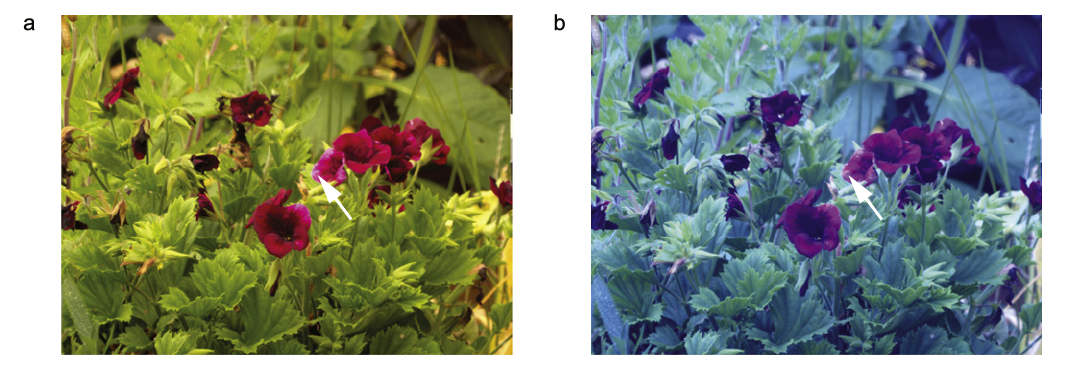
\includegraphics[max width=\textwidth]{figs/LitRev/fosterflowers.png}
% \caption{A single scene under two illuminants (\Gls{CCT} = 4000k and 25000K), reproduced from \citet{foster_color_2011}.}
% \label{fig:fosterflowers}
% \end{figure}

% \begin{figure}[htbp]
% 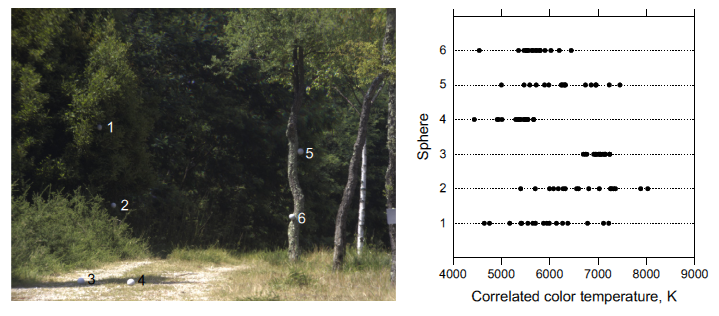
\includegraphics[max width=\textwidth]{figs/LitRev/greyballs.png}
% \caption{Reproduced from \citet{nascimento_spatial_2014}. Original figure caption: ``The color rendition on the left shows the scene with six embedded probe spheres indicated by numbers. The dot plot [on the right] shows the distribution of the CCTs of the local illumination at the 17 sample points on each of the spheres.''}
% \label{fig:greyballs}
% \end{figure}

%Figure \ref{fig:greyballs} gives an indication of the extent to which an object (or more precisely in this case, a group of nominally identical objects) can have varying colorimetric attributes across relatively minor spatial variation. 
%KC: This reads oddly to me, as it's more the illuminance that's varying than the object (if I've understood?).  I'd rephrase this.

% \begin{figure}[htbp]
% \includegraphics[max width=\textwidth]{figs/LitRev/X.png}
% \caption{\hl{Figure showing variation over time.}}
% \label{fig:X}
% \end{figure}

% Figure \ref{fig:fosterflowers} shows a single scene under illumination of two different \glspl{CCT}. The appearance of the object under the two illuminants is likely to have remained somewhat stable to an observer within the real scene, with observers choosing similar colour names for the object under each condition\footnote{Of course the appearance here, with these two images side-by-side, highlights the differences between the two conditions, and shows that under a single state of adaptation there is a clear distinction.}. 


% \subsubsection{Can chromatic adaptation fully account for colour constancy?}

% It may at first appear as though chromatic adaptation may be able to fully account for colour constancy

% RGB heuristic
% yes - cornsweet
% mechanistic vs inferential


% A similar level of variation occurs across time, for example as the sun passes behind a cloud.

% And so we have the central problem of colour constancy and chromatic adaptation: objects of which we have stable colour perceptions are able to be variant in both radiometric and colorimetric attributes without losing their apparent stability. The study of colour constancy aims to answer many questions which revolve around this central conundrum.

% Traditionally %(pre-1986, when \citet{arend_simultaneous_1986} performed what \citet{foster_color_2011} refers to as `the first systematic behavioral experiments' on color constancy) 
% there have existed two stances regards the nature of colour constancy; one held that it was enabled by adaptation of the sensory system, and the other that it was the result of unconscious inference. %KC: citation required
% It is my understanding that whilst great progress has been made in the intervening three decades, this is still a central question, although it appears to be widely accepted that the two frameworks might be complementary rather than mutually exclusive. %KC: citation required

%The best justification for their separation is perhaps that success in their study might serve different aims. 
%The first, the prediction of colour appearance, serves to further the utility of colour science, in particular colour appearance modelling, and the other systems which rely upon colour appearance modelling, such as colour difference formulation. 
%The second is best considered a vision science problem, concerned as it is with the function of the human visual organ, and advancement might endow us with an extension in our understanding of the human body. This in turn would have benefit in multiple areas, including feeding back to the prior aim, for once we understand the underlying mechanics we stand a much better chance of creating robust predictors of colour appearance. 
%Of particular interest to this author, understanding the underlying mechanisms of colour constancy should allow for a more intelligent design of lighting for the spaces which we inhabit, considering that artificial lighting need only resemble natural lighting to the extent that the visual system treats it as similar enough. Creating a colorimetric match to a specific spectra such as D65 is relatively easy, but until chromatic adaptation is more thoroughly understood it is not necessarily entirely clear what the appearance of such a match, or objects illuminated by it, might be. 

%The investigation of \glspl{CAT} generally occurs through the fitting of algorithms to data of corresponding colours, collected in varying manners, such that corresponding colours might be predicted for specific situations. The principal divides between the types of \gls{CAT} tend to hinge upon the method used to collect the data. \citet{nayatani_development_2006} divides the set as those derived from chromatic adaptation theory and those derived from fitting to experimental data, whereas Luo44 makes the divide between those studies based on aperture based experimental procedures and non-aperture based experimental procedures (which generally incorporate more complex, and therefore arguably more realistic, stimuli). Both parties use the terms `CAT Type I/II' to refer to these distinctions, but it is not entirely clear whether their distinctions are complementary. 

% This duality %get rid of this bollocks
% is mirrored by Foster37 in his discussion of the experimental methods employed in colour constancy research where he describes fundamental differences between those experiments which probe chromatic adaptation by asking observers to make `paper matches' (make it look like these two patches were cut from the same sheet of paper) and h/s/b matches (where observers are asked to match appearance in a non-relational manner, that is to match the qualia of a stimuli). This duality occurs again in Foster's37 comparison of relational and non-relational colour constancy, where relational refers to the maintaining of colour relationships in a scene and non-relational again refers to abstracted stimuli qualia). It is my suspicion that all of these disparate dualities are representations of the fundamental duality considered at the beginning of this chapter; that of a distinction between sensory adaptation and inferential computation.
